\chapter{\emph{Text scanning}}


\citet{1972_Knuth} describen dos tipos de programa que no
«submit gracefully to the new prohibition». Al organizar la
lectura de marcadores textuales, \citet[p. 271]{1974_Knuth}
se topa con un ejemplo parecido al siguiente.

\begin{minipage}{.6\linewidth}
\begin{center}
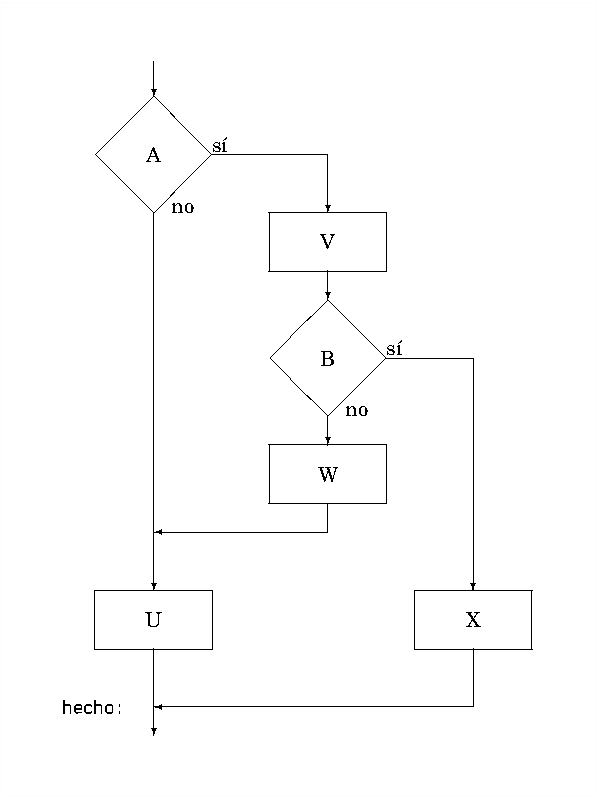
\includegraphics[scale=.8]{diagrama}
\end{center}
\end{minipage}
\hfill
\begin{minipage}{.3\linewidth}
\begin{center}
\NoCaptionOfAlgo
\begin{algorithm}[H]
\caption{con}
\SetKw{goto}{goto}
\DontPrintSemicolon
\If{A}{
  V\;
  \eIf{B}{
  X\;
  \goto \texttt{hecho}\;}{
  W\;}
}
U\;
\texttt{hecho:}
\end{algorithm}
\end{center}
\end{minipage}

¿Podríamos librarnos del «goto» sin duplicar código?

\NoCaptionOfAlgo
\begin{algorithm}[H]
\caption{sin}
\DontPrintSemicolon
\eIf{A}{
  V\;
  \eIf{B}{
    X\;}{
    W\;
    U\;
  }
}{
  U\;
}
\end{algorithm}
\vspace{5mm}

\lipsum[39-41]

\begin{figure}[ht!]
\begin{center}
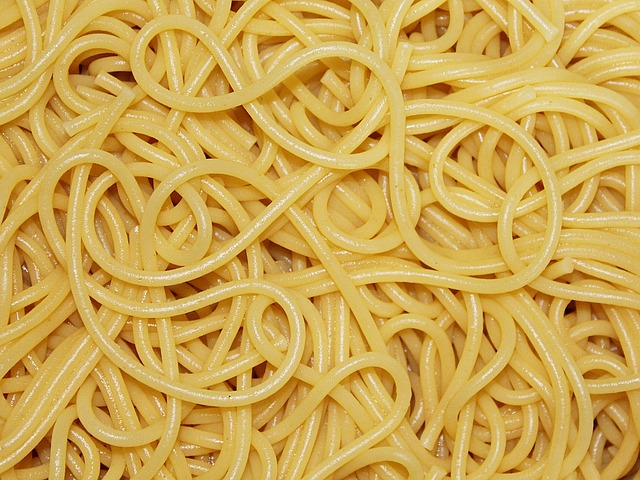
\includegraphics[width=\linewidth]{espaguetis}
\caption{}
\end{center}
\end{figure}

\lipsum[42-43]

\begin{figure}[ht!]
\begin{center}
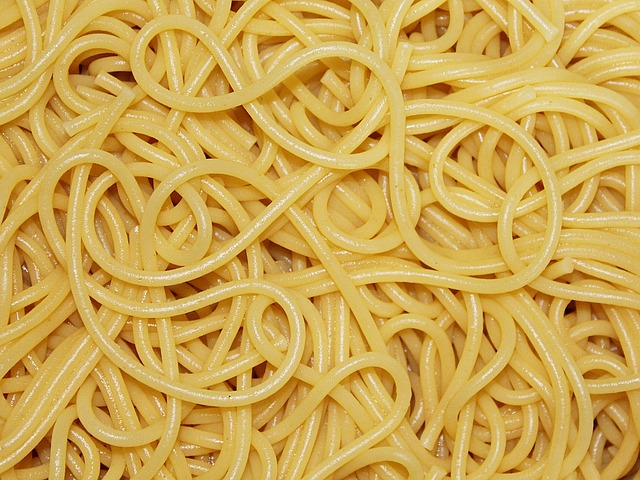
\includegraphics[width=\linewidth]{espaguetis}
\caption*{Sin número}
\end{center}
\end{figure}

\lipsum[45]
